\section{Versuchsaufbau}
\label{sec:aufbau}

	\begin{wrapfigure}{r}{7cm}
		\centering
		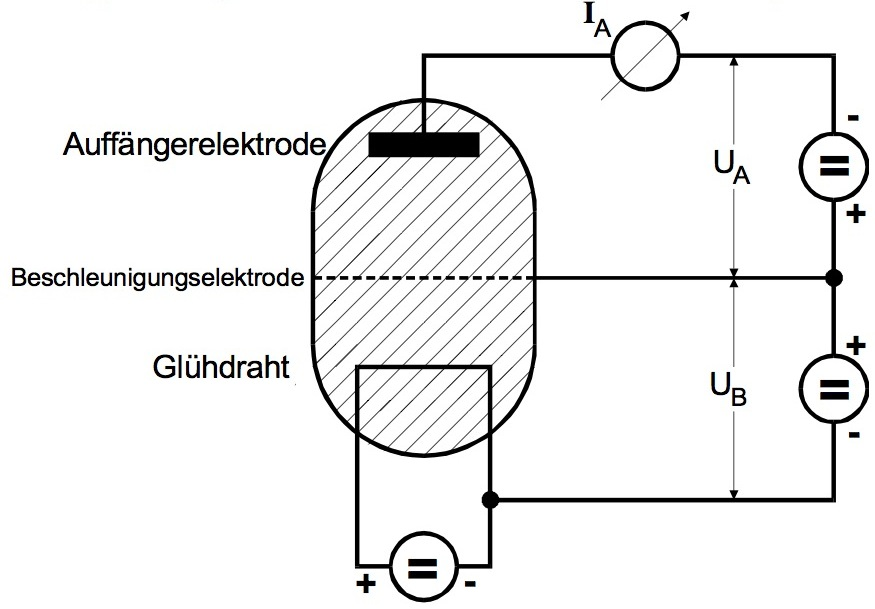
\includegraphics[width = 7cm]{img/aufbau.jpeg}
		\caption{Versuchsaufbau \cite{anleitung}. \label{fig:aufbau}}
	\end{wrapfigure}
	Der Franck-Hertz-Versuch ist in Abbildung \ref{fig:aufbau} schematisch Dargestellt.
	In einem evakuierten Gef"a"s verdampft ein Tropfen Quecksilber, sodass sich Quecksilberatome homogen in diesem verteilen.
	Der Druck des Quecksilberdampfes kann durch die Temperatur $T$ gesteuert werden.

	Im unteren Teil des Gef"a"ses befindet sich eine Gl"uhkathode aus Wolfram, die durch Gleichstrom erhitzt wird.
	Es treten auf Grund des gl"uhelektrischen Effektes Elektronen aus dem Material aus und bilden eine Elektronenwolke um den Wolframdraht.

	Zwischen Gl"uhkathode und einem, in der Mitte des Gef"a"ses befestigtem Drahtgitter, wird eine Spannung $U_\mathrm{B}$ angelegt, sodass die Elektronen in Richtung des Drahtgitters beschleunigt werden.

	Hinter dem Drahtgitter, im oberen Teil des Gef"a"ses befindet sich eine weitere Elektrode, die zum Drahtgitter ein negatives Potential $U_\mathrm{A}$ besitzt.
	Elektronen, die das Drahtgitter passieren und gen"ugend Energie besitzten, k"onnen das Potential $U_\mathrm{A}$ "uberwinden und als Auff"angerstrom $I_\mathrm{A}$ in der Elektrode gemessen werden.
	Langsame Elektronen werden dagegen zur"uck zum Drahtgitter gelenkt und von diesem absorbiert. 
	\\*

	\begin{wrapfigure}{r}{7cm}
		\centering
		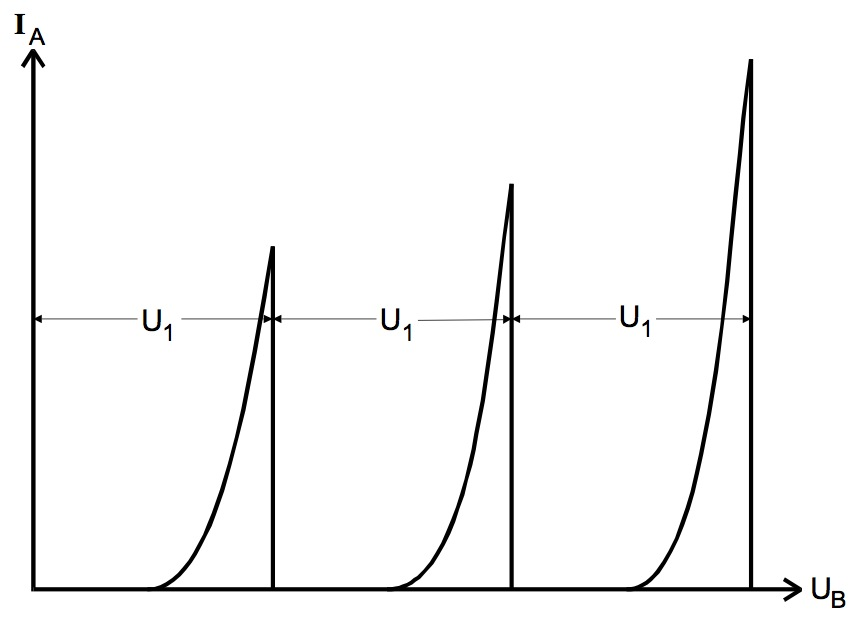
\includegraphics[width = 7cm]{img/strom-spannung.jpeg}
		\caption{Idealisiertes Strom-Spannungs-Diagramm \cite{anleitung}. \label{fig:strom-spannung}}
	\end{wrapfigure}

	Durch Erh"ohung der Beschleunigungsspannung $U_\mathrm{B}$ kann die kinetische Energie der Elektronen stetig erh"oht werden. Mit der Elektronenladung $e$ gilt
	\begin{equation}
		E_\mathrm{kin} = e \cdot U_\mathrm{B} \,.
	\end{equation}

	Bei konstanter Auff"angerspannung $U_\mathrm{A}$ erreichen dann mit steigender Spannung $U_\mathrm{B}$ immer mehr Elektronen die Auff"angerelektrode und der Strom $I_\mathrm{A}$ w"achst.

	Auf dem Weg durch das Gef"a"s sto"sen die Elektronen mit den Quecksilberatomen zusammen.
	Wenn sie nun gen"ugend kinetische Energie $E_\mathrm{kin} = \Delta E$ besitzen, sodass sie die Quecksilberatome anregen k"onnen, treten unelastische St"o"se auf.
	Die gesamte Energie der Elektronen geht dann in die Quecksilberatome "uber und der Strom $I_\mathrm{A}$ f"allt auf 0.
	Die kinetische Energie der Elektronen stimmt dann mit der Energiedifferenz $\Delta E$ zwischen Grundzustand und erstem angeregten Zustand des Quecksilberatoms "uberein.

	Durch weitere Erh"ohung der Beschleunigungsspannung $U_\mathrm{B}$ wiederholt sich dieser Prozess, sodass ein Strom-Spannungs-Diagramm, wie in Abbildung \ref{fig:strom-spannung} dargestellt, entsteht.
	Durch Messung des Abstandes $U_1$ zwischen zwei Strommaxima l"asst sich somit die Energiedifferenz $\Delta E$ bestimmen und es gilt

	\begin{equation}
		\Delta E = e \cdot U_1 \,. \label{eqn:anregung}
	\end{equation}

	\subsection{Systematische Abweichungen}
	\label{subsec:abweichungen}
		Auf Grund verschiedener Effekte, die im Folgenden aufgef"uhrt sind, weicht die tats"achlich messbare Kurve von der idealisierten Kurve in Abbildung \ref{fig:strom-spannung} ab.

		\begin{itemize}
			\item Die Strom-Spannungs-Kuver ist um einen Wert $K$ verschoben.
			Dieser Wert $K$ bezeichnet das Kontaktpotential, welches auf Grund der verschiedenen Austrittsarbeiten des Kathoden- und des Gitterdrahtmaterials auftritt und durch das Fermi-Niveau $\Phi$ der Materialien bestimmt ist:

			\begin{equation*}
				K = \frac{1}{e} (\Phi_\mathrm{B} - \Phi_\mathrm{A}) \label{eqn:k}
			\end{equation*}

			\item Die Kurve erscheint abgeflacht und verbreitert, weil die Elektronen nicht mit konstanter Geschwindigkeit aus dem Gl"uhdraht austreten.
			Die Elektronen besitzen stattdessen ein Energiespektrum, welches als Fermi-Dirac-Verteilung bezeichnet wird.
			Dadurch f"allt der Auff"angerstrom $I_\mathrm{A}$ nach einem Maximum nicht mehr unstetig auf den Wert 0 ab, sondern n"ahert sich stetig einem Minumum, das nicht 0 ist.

			\item Die Wahrscheinlichkeit, dass die Elektronen mit Quecksilberatomen kollidieren h"angt stark vom S"attigungsdampfdruck $p_\mathrm{s"at}$ des Quecksilbergases ab.
			Dieser legt die freie Wegl"ange $\overline{w}$ fest, die ein Elektron durchschnittlich zur"ucklegen muss, um mit einem Quecksilberatom zu kollidieren.
			Es gilt

			\begin{eqnarray}
				\label{eqn:w} \overline{w} & = & \frac{\SI{.0029}{}}{p_\mathrm{s"at}} \,, \\
				\label{eqn:p} p_\mathrm{s"at}(T) & = & \SI{5.5e7}{} e^{\SI{-6876}{} / T} \,.
			\end{eqnarray}

			Der Druck $p_\mathrm{s"at}$ wird dabei in Millibar, die freie Wegl"ange $\overline{w}$ in Zentimeter angegeben.

			Falls die Wegl"ange $\overline{w}$ gr"o"ser als die Dimension $a$ der Versuchsapparatur ist, treten kaum Kollisionen auf und eine Messung ist schwierig.
			Wenn die Wegl"ange $\overline{w}$ viel kleiner ist als $a$, treten zwischen den unelastischen St"o"sen viele elastische St"o"se auf, die mit starken Richtungs"anderungen verbunden sind.
			Dadurch verringert sich die Anzahl der Elektronen, die die Auffangelektrode erreichen und das Ergebnis wird verf"alscht.
		\end{itemize}

	\clearpage

\section{Durchf"uhrung}
\label{sec:durchfuehrung}
	\begin{figure}[h]
		\centering
		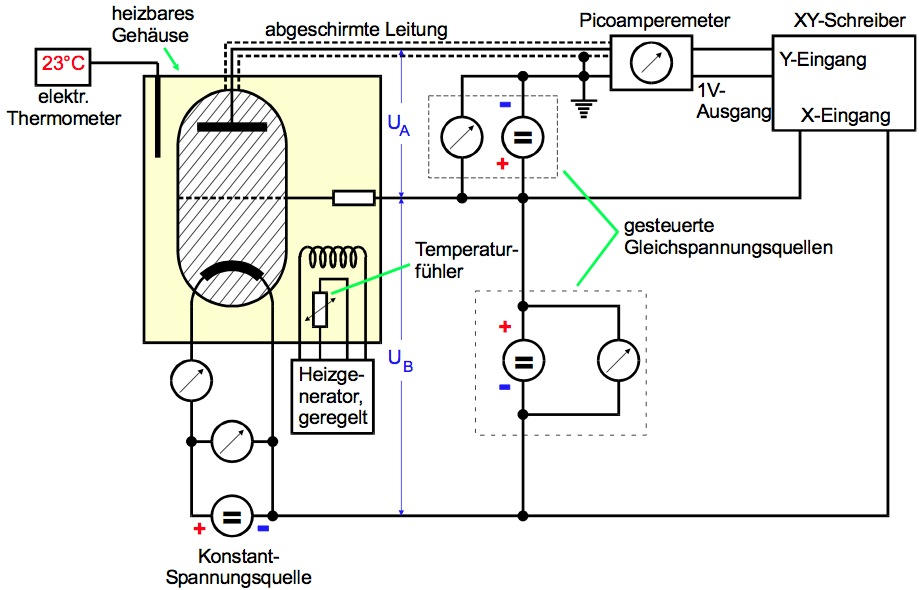
\includegraphics[width = 12cm]{img/aufbau-exakt.jpeg}
		\caption{Aufbau der hier verwendeten Apparatur \cite{anleitung}. \label{fig:aufbau-exakt}}
	\end{figure}

	Die hier verwendete Apparatur ist in Abbildung \ref{fig:aufbau-exakt} dargestellt.
	Das gesamte, mit Quecksilberdampf bef"ullte Gef"a"s befindet sich in einem Blechgeh"ause, welches durch einen elektronischen Temperaturregler erhitzt werden kann.
	Die Temperatur $T$ wird mit einem elektronischen Thermometer gemessen.
	Die Brems- und Beschleunigungsspannungen $U_\mathrm{A}$ und $U_\mathrm{B}$ k"onnen kontinuierlich zwischen 0 und $U_\mathrm{A} = \SI{11}{\volt}$ bzw. $U_\mathrm{B} = \SI{60}{\volt}$ geregelt werden.
	Dabei kann die Zeit $t$, in der die Spannung geregelt wird, zwischen $t = \SI{30}{\second}$ und $t = \SI{5}{\minute}$ variiert werden.

	Der XY-Schreiber muss vor der ersten Messung justiert werden, indem ohne Eingangssignal der Nullpunkt beider Richtungen auf den Nullpunkt der Skalierung eingestellt wird.
	Der Y-Eingang wird dann mit dem Signal des Picoamperemeters, welches den Auff"angerstrom $I_\mathrm{A}$ misst, gespeist, 
	der X-Eingang wahlweise mit der Spannung $U_\mathrm{A}$ oder $U_\mathrm{B}$.

	Vor jeder Messung m"ussen die maximalen Werte f"ur Strom und Spannung eingestellt werden, sodass die Auslenkungen des XY-Schreibers f"ur diese ebenfalls maximiert werden k"onnen.
	Dadurch ist sichergestellt, dass der XY-Schreiber nicht "uberregelt.
	\\*

	Zuerst wird die integrale Energieverteilung der beschleunigten Elektronen bestimmt.
	Dazu wird der Auff"angerstrom $I_\mathrm{A}$ in Abh"angigkeit der Bremsspannung $U_\mathrm{A}$ bei konstanter Beschleunigungsspannung $U_\mathrm{B} = \SI{11}{\volt}$ gemessen.
	Diese Messung wird bei Zimmertemperatur $T \approx \SI{20}{\celsius}$ und bei einer erh"ohten Temperatur $T \approx \SI{150}{\celsius}$ durchgef"uhrt.
	Aus dem Diagramm bei Zimmertemperatur l"asst sich dann das Kontaktpotential $K$ ablesen.
	\\*

	Anschlie"send wird bei einer Temperatur von $T \approx \SI{180}{\celsius}$ eine Frank-Hertz-Kurve aufgenommen.
	Dazu wird bei konstanter Auff"angerspannung $U_\mathrm{A} \approx \SI{1}{\volt}$ die Beschleunigungsspannung $U_\mathrm{B}$ von 0 auf $U_\mathrm{B} = \SI{60}{\volt}$ geregelt.
	Aus der Kurve kann dann durch Abstandsmessung der Maxima die Energiedifferenz $\Delta E$ aus Kapitel \ref{subsec:ww} bestimmt werden.
	\\*

	Schlie"slich wird bei einer Temperatur $T \approx \SI{105}{\celsius}$ und einer Auff"angerspannung $U_\mathrm{A} = \SI{-30}{\volt}$ der Auff"angerstrom $I_\mathrm{A}$ gemessen.
	Dabei ist darauf zu achten, dass die Polung des Y-Eingangs sowie des Picoamperemeters getauscht werden muss.
	Der Strom $I_\mathrm{A}$ ist hierbei zun"achst nicht messbar und steigt ab einer Bestimmten Spannung $U$ stark, nahezu sprunghaft an.
	Durch extrapolation dieser Kurve auf den Wert $I_\mathrm{A} = 0$ l"asst sich dann die Ionisationsspannung $U_\mathrm{ion}$ und damit die Ionisationsenergie $E_\mathrm{ion}$ f"ur Quecksilber bestimmen:

	\begin{equation}
		E_\mathrm{ion} = e \cdot U_\mathrm{ion}
	\end{equation}